Deteksi manusia dan barang merupakan kemampuan yang sangat diperlukan di berbagai teknologi saat ini, tidak hanya robot. Hal ini dikarenakan banyaknya manfaat yang didapat dari pengembangannya untuk diaplikasikan menjadi fungsi lain. Berbagai metode dikembangkan untuk membangun sistem deteksi manusia dan barang. Bermacam-macam jenis sensor dilibatkan supaya dapat memberikan hasil yang bagus. Penggunaan \lidar\ untuk deteksi ini memberi keuntungan yaitu komputasi lebih rendah dengan akurasi sensor yang baik. Selain itu, pengguna tidak perlu memasangkan sensor pada target karena perangkat \lidar\ memancarkan pulsa sinar laser yang cepat dan mengukur jumlah waktu yang diperlukan untuk setiap pulsa yang memantul kembali untuk menentukan jarak target.

\section{Analisis Metode \textit{Leg Detection}}
\label{sec:Metode_02}

    Metode \textit{leg detection} (LD) mendeteksi manusia dengan melalui bagian kaki manusia sehingga \lidar\ diletakkan pada posisi yang cukup rendah yaitu $\pm 30$ cm sampai $50$ cm dari permukaan tanah untuk mendeteksi objek\cite{c1}. Metode ini sudah pernah dikembangkan pada ROS sehingga ROS sudah memiliki \textit{package} untuk LD, contohnya paket \textit{cob\_ people\_ perception} memungkinkan untuk menemukan pola berbentuk kaki dari pembacaan laser. Paket ini sayangnya sudah tidak dapat diakses lagi. Metode LD yang lainnya adalah metode pendeteksian kaki yang menggunakan beberapa sensor statis yang tersebar kemudian menggabungkannya dengan sistem jaringan dan server. Metode tersebut tidak dapat diterapkan pada proyek \capstone\ ini karena memerlukan sensor lebih dari satu dan sensor tidak bisa terpasang pada robot. Hal ini berarti metode pendeteksi kaki yang dapat diaplikasikan dan dikembangkan pada proyek ini adalah metode yang menggunakan sebuah sensor yang diletakkan pada robot. 

    Contoh metode LD dengan sensor pada robot yang telah berhasil dikembangkan adalah \textit{PeTra} yang dibuat oleh klub robotika \textit{University of León}. Sistem ini menggunakan pesan masukkan dari pemindai \lidar\ dan menggunakan data terlatih untuk mengklasifikasikan kelompok yang dideteksi termasuk kaki atau bukan. Deteksi dilakukan oleh \textit{classifier} menggunakan algoritma \textit{Random Trees} yang diimplementasikan dengan API OpenCV. \textit{Training data} diperoleh dengan mengumpulkan data dari satu orang yang berjalan dalam garis lurus menuju robot dan kemudian berbalik untuk menjauhi robot yang berada dalam kondisi tetap diam. Proyek ini belum menerima pengembangan berkelanjutan dan tidak ada versi perangkat lunak untuk versi ROS terbaru. 

    Metode lain pengembangan LD yang saat ini banyak dilakukan adalah dengan sensor berada di robot untuk mendeteksi bentuk geometri kaki manusia. Metode ini dikembangkan untuk mendeteksi banyak manusia berjalan dari suatu robot bergerak. Biasanya metode ini dikembangkan untuk melacak orang-orang yang hanya mengenakan celana agar bentuk geometris kaki lebih mudah dibedakan dari objek lain.
    % Penggunaan karakteristik geometris kaki manusia dan frekuensi-fase gerakan berjalan telah diuji (Lee et al., 2006), tetapi tidak dapat menangani oklusi parsial, perubahan kecepatan orang, dsb. Sensor akan memindai seluruh objek sehingga benda-benda seperti meja atau kaki kursi, batang tanaman, dll., mungkin mudah dikacaukan dengan kaki orang. Juga sulit untuk melacak orang tertentu (sepasang kaki) di lingkungan yang ramai karena banyak tabrakan dapat terjadi.
    Kesulitan utamanya berasal dari \textit{uncertainty} dan \textit{noise} data sensor karena objek yang dilacak dan juga sensor pada robot akan bergerak dalam aplikasi situasi nyata. Selain itu, terjadi beberapa oklusi yang terjadi saat pemindaian objek lain, selain itu kadang-kadang salah satu dari dua kaki tidak dapat dideteksi sesuai dengan arah gerakan berjalan manusia. Solusi untuk mengatasi masalah tersebut yaitu dengan menggunakan Extended Kalman Filter untuk memodelkan manusia yang berjalan.
    %
    % They used multiple static LRF sensors
    % attached on the ground and combined them with network and
    % server system. The method is extended for using both LRF
    % and vision[8,10].
    %
    % Different solutions have been proposed previously in the literature to deal with the problem of tracking people using a 2D LIDAR scanner mounted on a mobile robot. Navigation in peopled, mapped, indoor environments has been recently reviewed (Rios-Martinez et al., 2015). 
    %
    % The use of the geometric characteristics of human legs and the frequency and phase of walking motion have been tested (Lee et al., 2006), but cannot deal with partial occlusions, changes in peoples' speed, etc. In this article we are concerned with the specific problem of detecting pairs of legs (from a person) and being able to track them.
    %
    % The charm point of the approach of this paper is to track multiple walking humans from a ``moving'' robot with walking model. Its principal difficulties come from the uncertainty and noise of sensor data, because not only the object being tracked but also the sensor on a robot is moving in real applications. Moreover, there happen some occlusions owing to screening by another object, and sometimes one of two legs cannot be detected according to the direction of human walking motion. These also increase the uncertainty of extracted human data. To cope with those difficulties, human walking model with Extended Kalman Filter is utilized.
    % Tracking procedure is designed as following sequences that are iterated every scanning time. In this research, it is assumed that we track people putting on just general trousers, excepting skirt or other dressing style, and the knee part of human leg is scanned.:
    Prosedur \textit{tracking} ini dirancang dari beberapa tahap yang terus diulang-ulang setiap pemindaian. Berikut adalah langkah-langkah yang ditempuh untuk metode LD dengan sensor pada robot\cite{c1b}:
    \begin{enumerate}
        \item Pengelompokan Data: Hal ini diperlukan untuk mengekstrak data orang berjalan dari data pemindaian sensor yang berupa data mentah dengan informasi baik dari orang-orang maupun lingkungan. Data hasil pemindaian dibagi menjadi beberapa cluster dan cluster yang ukurannya mirip kaki manusia (lebar kurang dari 25 cm) diklasifikasikan menjadi kandidat kaki.
        % Data Clustering: Firstly, it is needed to extract the data of walking people from the scanning data from LRF sensor because raw data has information of both people and environments. 

        \begin{figure}[H]
            \centering
            \begin{subfigure}[b]{.30\textwidth}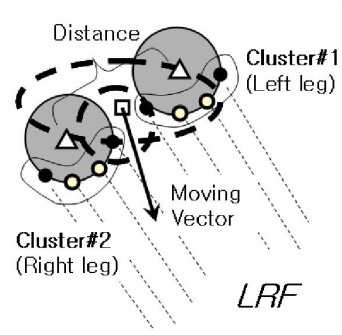
\includegraphics[width=\linewidth]{bab3/leg_detection1.png}\caption{Dua Kaki Manusia}\label{Fig:Ch02_leg1}\end{subfigure}
            \begin{subfigure}[b]{.30\textwidth}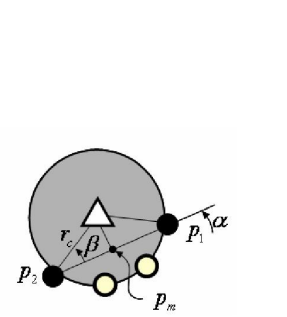
\includegraphics[width=\linewidth]{bab3/section_leg.png}\caption{Satu Kaki Manusia}\label{Fig:Ch02_leg2}\end{subfigure}
            \caption{Tampilan Data Kaki Manusia dari Atas\cite{c1b}.}
            \label{Fig:ch02_posisi_leg}
        \end{figure}
        \item Proses Menemukan Posisi Kaki: selanjutnya, posisi bagian tengah kaki harus dihitung karena kandidat kaki yang diberikan dari proses pengelompokan sebelumnya hanya memiliki bagian kaki seperti yang ditampilkan pada Gambar \ref{Fig:Ch02_leg1}. 
        % Finding Leg Position: Next, the center of leg section should be computed because leg candidate given from previous clustering process has just a part of leg section as displayed in Fig. 2 (a). 
        Gambar \ref{Fig:Ch02_leg2} menunjukkan satu lingkar kaki dimana lingkaran kecil menunjukkan titik-titik dipindai oleh sensor jarak dengan $p_1$ dan$p_2$ adalah titik awal dan akhir dari kandidat kaki. 
        Posisi tengah bagian kaki adalah dihitung dengan mempertimbangkan geometri kaki dengan persamaan berikut.
        \begin{equation}
            \begin{pmatrix}
                x_{leg}\\
                y_{leg}
            \end{pmatrix} =
            \begin{pmatrix}
                x_{p2}\\
                y_{p2}
            \end{pmatrix} +
            \begin{pmatrix}
                \glsadd{r_c}
                r_c\glsadd{r_c} \cos (\alpha + \beta)\\
                r_c\glsadd{r_c} \sin (\alpha + \beta)
            \end{pmatrix}
        \end{equation}
        dimana $p_1, p_2 $ dan $r_c\glsadd{r_c}$ menunjukkan titik pertama kaki, terakhir dari kaki, dan jari-jari kaki yang diasumsikan $\pm 7$ cm, kemudian dihitung titik tengah kaki $(x_{leg},y_{leg})$.

        \item Proses Menghubungkan Posisi Manusia dengan Kandidat Kaki: Kandidat kaki yang dibuat pada langkah pengelompokan sebelumnya digunakan sebagai posisi baru manusia berjalan, sehingga objek manusia dengan dua kaki yang dibuat pada pemindaian sebelumnya terhubung dengan kandidat kaki baru.
        % Connecting Human Objects to Leg Candidates: Leg candidates made in previous clustering step are used as the new position of walking human. Thus, human objects created in the past scanning time have two legs, and both of them are connected with new leg candidates. 
        \item Pembuatan Objek Manusia Baru: Objek manusia yang baru akan dibuat dari kandidat kaki lainnya yang tidak terhubung ke objek manusia yang ada dalam prosedur penghubungan sebelumnya. Sepasang kandidat kaki yang jaraknya di antara mereka lebih pendek dari langkah normal ($<50$ cm) menjadi objek manusia baru.
        % Creating New Human Object: New human object are created from the rest of leg candidates which are not connected to the existing human objects in the previous connecting procedure. A pair of leg candidates whose distance between them is shorter than that of normal stride(<50cm) becomes a new human object.
        \item \textit{Update} Objek Manusia: Keadaan objek manusia di-\textit{update} menggunakan model berjalan manusia dengan data posisi diberikan dari prosedur sebelumnya. Beberapa objek manusia tanpa data posisi baru dari waktu pemindaian ini juga diperbarui dengan prediksi. Kandidat kaki baru yang belum terhubung ke objek manusia sebagai data pemindaian baru, maka sementara waktu akan dikategorikan sebagai keadaan oklusi. Data tersebut akan dihilangkan jika waktu oklusi objek manusia melebihi nilai yang diberikan.
        % Update Human Objects: The states of human objects are updated using human walking model with the measured position data given from previous procedures. Some human objects without new position data from this scanning time are also updated with just prediction. If new leg candidate has not been connected to a human object as new scanning data for a while, it means occlusion state. If occlusion time of a human object exceeds a given value, we consider it as disappearance and delete it. And states of another objects created in this scanning time are initialized. Walking model used in this paper will be discussed in detail in the next chapter.
        \item Pemindaian Berikutnya: Setelah proses selesai, maka akan dilanjutkan proses pemindaian selanjutnya dengan data baru yang diterima sensor.
    \end{enumerate}

\section{Analisis Metode \textit{Torso Detection}}
\label{sec:Metode_03}

    % In supervised machine learning, a group of labelled samples is the training data with known category, and the model learns from the correctly identified samples. 

    Metode ini memanfaatkan bentuk \textit{elips} untuk melacak bagian dada manusia kemudian menentukan objek terdeteksi merupakan manusia atau bukan\cite{c2}. Dada memiliki bentuk yang lebih sederhana dan tidak banyak mengalami perubahan ketika aktivitas. Seperti pendeteksian pada umumnya, masalah pendeteksian ditangani dengan memanfaatkan algoritma klasifikasi. Pengamatan individu yang diubah menjadi properti yang dapat diukur dikenal sebagai fitur. Algoritma yang melakukan klasifikasi disebut pengklasifikasi/\textit{classifier}. Pemilihan \textit{classifier} merupakan bagian penting dalam proses deteksi.

    Langkah pertama dilakukan segmentasi data berdasarkan pada pendeteksian titik-titik diskontinuitas dalam pemindaian laser. Laser mencapai jangkauan dan arah $\{r_i, \theta\glsadd{theta}_i \}$ sejauh objek dalam bidang pandangnya dengan $i$ bernilai $i = 1......n.$. Segmentasi dilakukan dengan menggunakan teknik \textit{model based} yang direalisasikan menggunakan \textit{Extended Kalman Filter} (EKF) \cite{c4}, data dapat dipartisi menjadi segmen-segmen $S = \{s_1, s_2, ,...,s_M\}$ seperti pada Gambar \ref{fig:Ch03_segmentasi}.
        
        \begin{figure}[H]
            \centering
            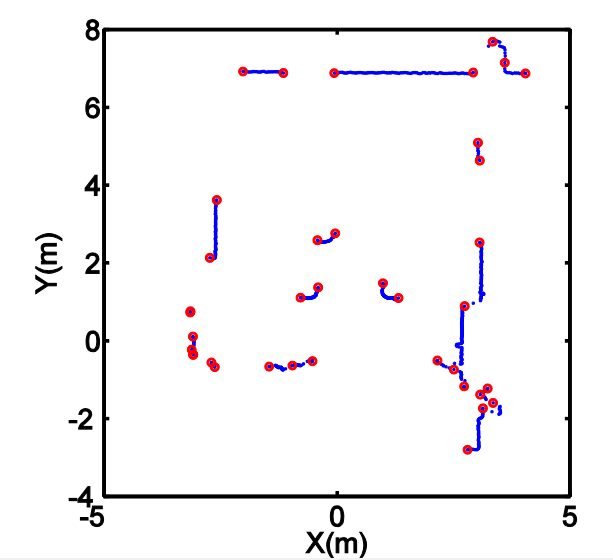
\includegraphics[scale=0.35]{segmentasi.png}
            \caption{\textit{Plotting} segmentasi bacaan \lidar\cite{c2}.}
            \label{fig:Ch03_segmentasi}
        \end{figure}

        Langkah selanjutnya setelah melakukan segmentasi adalah ekstraksi fitur-fitur yang akan digunakan dalam deteksi manusia. Fitur pertama adalah panjang segmen yang diperoleh dari persamaan berikut:
        \begin{equation}
            \sqrt{(x_n-x_1)^2+(y_n-y_1)^2}
        \end{equation} 
        dengan panjang segmen dihitung dari titik awal $(x_1,y_1)$ hingga titik $akhir (x_n,y_n)$. Fitur kedua yang dicari adalah rasio sumbu mayor dan minor elips. 
        \textit{Cross section} dada manusia umumnya dapat diperkirakan dengan elips. Oleh karena itu, algoritma elips diimplementasikan pada hasil segmentasi. Fitur ketiga yang dicari adalah \textit{mean} karakteristik kurva dari segmen. Nilai perkiraan kelengkungan diskrit dari kurva adalah\cite{c2b}:
        \begin{equation}
            k=\frac{4A}{d_1d_cd_n}
        \end{equation}
        dengan $d_1, d_c, d_n$ merupakan jarak antar titik $x_1, x_n, x_c\glsadd{x_c}$ yang diperoleh dari titik awal kurva, titik akhir kurva, dan titik tengah kurva, kemudian $A$ adalah area di dalam ketiga titik tersebut. 
        Fitur keempat adalah rasio jarak antara sumber laser menuju pusat segmentasi dari sekumpulan titik yang dihitung:
        \begin{equation}
            \sqrt{\frac{x_c\glsadd{x_c}^2+y_c\glsadd{y_c}^2}{n}}
        \end{equation} 
        
        dengan $(x_c\glsadd{x_c},y_c\glsadd{y_c})$ adalah pusat segmen dan $n$ adalah jumlah titik.

    Langkah selanjutnya adalah melakukan ekstraksi fitur yang berupa panjang segmen, rasio antara sumbu mayor dan sumbu minor elips, karakteristik kelengkungan segmen, dan jarak antara sumber laser dengan pusat segmen. Setelah itu dilakukan klasifikasi menggunakan \textit{Radial Basis Function Support Vector Machines} (RBFSVM) yang dituliskan menjadi fungsi kernel:
    \begin{equation}
        K(\mathbf{F_i,F_j})=exp(-\gamma||\mathbf{F_i}-\mathbf{F_j}||^2), \gamma >0,
    \end{equation}
    \begin{tabbing}
        dengan: \=\\
            \>$\mathbf{F_i}$ \qquad \=: \textit{training vectors i},\\ 
            \>$\mathbf{F_j}$ \>: \textit{training vectors j},\\
            \>$\gamma$ \>: parameter kernel.
    \end{tabbing}
    
\section{Analisis Metode \textit{Hip Detection}}
\label{sec:Metode_01}

    Metode ini menggunakan \lidar\ untuk membaca lingkungan dengan cara memancarkan pulsa sinar laser yang cepat, kemudian hasil bacaan \lidar\ perlu diubah ke dalam bentuk denah dua dimensi (2D). \lidar\ 2D lebih diutamakan untuk digunakan daripada \lidar\ 1D dan 3D untuk mencapai keseimbangan antara kompleksitas komputasi dan biaya rendah. Hasil bacaan mentah \lidar\ dikurangi jumlah dimensinya dengan ekstraksi. Kemudian pada fase tampilan, ditunjukkan berapa manusia yang terdeteksi pada denah output serta menghitung jumlahnya secara \textit{real-time}. Seperti yang terlihat pada Gambar \ref{fig:Ch02_Hip_Detec}, metode ini mengimplementasikan aplikasi untuk penghitungan dan pendeteksian orang dengan menempatkan LIDAR pada tingkat yang lebih tinggi (setinggi panggul)\cite{c3}. Target keluarannya yaitu membedakan manusia dari objek sekitarnya. 
    Fitur diperoleh dari data \lidar\ asli yang bertindak sebagai masukan untuk pelatihan atau prediksi model. Proses penurunan fitur dikenal sebagai ekstraksi fitur yang dilakukan untuk mengurangi jumlah dimensi. 
    
    \begin{figure}[H]
            \centering
            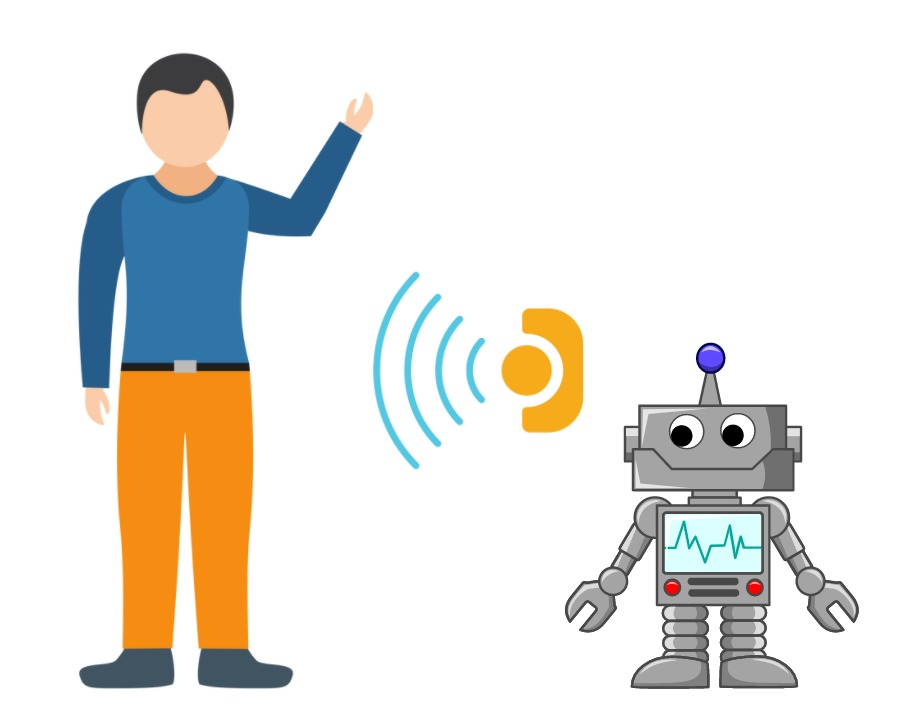
\includegraphics[scale=0.3]{Hip_detec.jpeg}
            \caption{Ilustrasi Metode \textit{Hip Detection}.}
            \label{fig:Ch02_Hip_Detec}
        \end{figure}
 
    Sebelum melakukan klasifikasi, data yang didapat perlu dikelompokkan. Teknik \textit{clustering} adalah teknik pengelompokan objek berdasarkan kesamaan karakteristiknya. Pengelompokan ini menggunakan metode Density-Based Spatial Clustering of Applications with Noise(DBSCAN). DBSCAN digunakan untuk mengelompokkan titik berdasarkan jarak menggunakan nilai  \textit{minimum points} (MinPts) dan epsilon ($\backepsilon$). $\backepsilon $ mendefinisikan radius lingkungan di sekitar titik $x$. MinPts adalah jumlah minimum tetangga dalam radius $\backepsilon$. Selanjutnya untuk memprediksi apakah \textit{cluster} termasuk manusia atau bukan manusia diperlukan algoritma klasifikasi yaitu menggunakan algoritma Random Forest. 
    
    Ukuran \textit{cluster}, perbedaan standar dari \textit{mean}, rata-rata perbedaan \textit{mean}, lebar, \textit{linearity}, \textit{circularity}, jari-jari, \textit{boundary regularity}, \textit{mean curvature},\textit{ angular difference, inscribed angular variance, standard inscribed angular variance}, jarak, dan jarak/ukuran \textit{cluster} adalah 14 fitur yang diekstraksi dari \textit{cluster}. Semua fitur ini diekstraksi dari setiap \textit{cluster} diperhitungkan untuk mengklasifikasikan sampel yang masuk.  Terakhir, pada fase tampilan ditunjukkan manusia yang terdeteksi serta menghitung secara \textit{real-time} melalui denah 2D dari data \lidar.

\section{Pemilihan Metode}
\label{sec:Pemilihan_Metode}

Pemilihan metode dapat menghasilkan hasil lebih maksimal
dengan memahami kelebihan dan kekurangan masing-masing metode. Berikut akan dibahas kelebihan dan kekurangan untuk masing-masing metode berdasarkan tabel kelebihan dan kekurangan masing-masing metode yang ditunjukkan pada Tabel \ref{tab:Ch05_Methods}.
\begin{longtable}{|c|L{1.8 cm}|L{4.8 cm}|L{4.8cm}|L{0.6cm}|}
   \caption{Kelebihan dan Kekurangan Metode-Metode Sistem Deteksi} 
   \label{tab:Ch05_Methods}
   \vspace{-0.75em}\\
   \hline
   \multicolumn{1}{|c|}{\textbf{No}} & \multicolumn{1}{|c|}{\textbf{Metode}}  & \multicolumn{1}{|c|}{\textbf{Kelebihan}} & \multicolumn{1}{|c|}{\textbf{Kekurangan}} & \multicolumn{1}{|c|}{\textbf{Total Skor}} \\ \hline
   1           & Leg Detection      &  \begin{tabular}[C{|c|}]{@{}L{4.5 cm}@{}}
       \begin{itemize}
           \item Sudah pernah dikembangkan pada ROS(+3).
           \item Letak \lidar\ rendah sehingga semua objek di sekitarnya dapat terbaca(+3).
       \end{itemize}
   \end{tabular}        & \begin{tabular}[C{|c|}]{@{}L{4.5 cm}@{}}
   \begin{itemize}
           \item \textit{Package} ROS sudah tidak dapat diakses dengan versi ROS terbaru(-2).
           \item algoritma lebih rumit ketika dikembangkan untuk \textit{tracking} jika jumlah kaki banyak(-1).
       \end{itemize}
   \end{tabular} 
   & \multicolumn{1}{|c|}{3}  \\ \hline
   2           & Torso Detection     & 
   \begin{tabular}[C{|c|}]{@{}L{4.5 cm}@{}}
       \begin{itemize}
           \item Bentuk torso tidak mengalami banyak perubahan dan banyak pergerakan(+2).
           \item Bentuk tidak serumit kaki manusia(+1).
       \end{itemize}
   \end{tabular}
   & \begin{tabular}[C{|c|}]{@{}L{4.5 cm}@{}}
       \begin{itemize}
           \item Pemasangan terlalu tinggi(-1).
           \item \textit{backscattering noise} yang diterima banyak karena \lidar\ dekat dengan sumber cahaya lainnya(-2).
       \end{itemize}
   \end{tabular}   
   & \multicolumn{1}{|c|}{0}  \\ \hline
   3           & Hip Detection & 
   \begin{tabular}[C{|c|}]{@{}L{4.5 cm}@{}}
       \begin{itemize}
           \item Bentuk sederhana(+2).
           \item Pemasangan \lidar\ tidak terlalu rendah atau tinggi(+2).
       \end{itemize}
   \end{tabular}        
   & \begin{tabular}[C{|c|}]{@{}L{4.5 cm}@{}}
       \begin{itemize}
           \item Sama dengan metode \textit{torso detection} namun dengan jumlah \textit{backscattering noise} lebih sedikit(-2).
       \end{itemize}
   \end{tabular} 
   & \multicolumn{1}{|c|}{2}  \\ \hline

\end{longtable}
    Pada Tabel \ref*{tab:Ch05_Methods} terlihat bahwa masing-masing metode memiliki skor untuk setiap poin kelebihan dan kekurangan. Terlihat antara metode-metode tersebut, nilai skor yang paling tinggi dimiliki metode LD. Penerapan metode ini memerlukan perancangan dari pemrosesan data mentah \lidar\ hingga pendeteksian. Bentuk geometri hasil pembacaan kaki manusia akan digunakan sebagai pembeda manusia dengan objek yang lainnya.
    
    Metode LD juga sesuai dengan rencana kondisi peletakan \lidar\ pada robot yaitu setinggi kaki. \lidar\ yang diletakkan pada posisi bawah robot akan lebih mudah memperoleh data data dibandingkan posisi peletakan yang lebih tinggi. Berbeda dengan metode awal \textit{hip detection}, metode ini lebih mudah diaplikasikan pada robot dikarenakan peletakan sensor dan proses pemindaian lingkungan tidak terganggu dengan bagian robot lainnya. Objek yang terdeteksi juga memiliki lebih sedikit variasi bentuk daripada objek-objek yang terbaca pada peletakan \lidar\ yang lebih tinggi.
    
    Oleh karena itu, metode yang digunakan adalah metode LD.
    Metode ini akan diimplementasikan secara sederhana yaitu dengan mendeteksi objek berupa lingkaran yang sesuai untuk mengidentifikasi kaki manusia. Objek-objek di sekitar akan dibedakan menjadi dua bentuk yaitu garis lurus dan lingkaran. Objek-objek lingkaran kemudian dikelompokkan yang memenuhi syarat sebagai kaki manusia lalu posisi manusia ditentukan dari kaki-kaki yang terdeteksi tersebut.


% Tracking peoples' legs using only information from a 2D LIDAR scanner in a mobile robot is a challenging problem because many legs can be present in an indoor environment, there are frequent occlusions and self-occlusions, many items in the environment such as table legs or columns could resemble legs as a result of the limited information provided by two-dimensional LIDAR usually mounted at knee height in mobile robots, etc. 

% for instance, the cob\_people\_perception package allows to find leg-like patterns of laser scanner readings. This software is based on the LD approach and implementation.\\
% It obtains incoming messages from the LIDAR scanner and uses trained data to classify the groups of laser records as possible legs. Detection is performed by a classifier using Random Trees implemented with the OpenCV API. However, LD has an important drawback; the project has not received continuous development and there is not a version of the software for the latest ROS versions.

% Metode ini menggunakan pesan masuk dari pemindai LIDAR dan menggunakan data terlatih untuk mengklasifikasikan kelompok termasuk kaki atau bukan. Deteksi dilakukan oleh \textit{classifier} menggunakan \textit{Random Trees} yang diimplementasikan dengan API OpenCV. Namun, proyek ini belum menerima pengembangan berkelanjutan dan tidak ada versi perangkat lunak untuk versi ROS terbaru.

